\documentclass[10pt, a4paper]{amsart}

\usepackage{graphicx}
\usepackage{hyperref}

% Augmented matrices.
\makeatletter
\renewcommand*\env@matrix[1][*\c@MaxMatrixCols c]{%
  \hskip -\arraycolsep
  \let\@ifnextchar\new@ifnextchar
  \array{#1}}
\makeatother

%--------grstep
% For denoting a Gauss' reduction step.
% Use as: \grstep{\rho_1+\rho_3} or \grstep[2\rho_5 \\ 3\rho_6]{\rho_1+\rho_3}
\newcommand{\grstep}[2][\relax]{%
   \ensuremath{\mathrel{
       {\mathop{\longrightarrow}\limits^{#2\mathstrut}_{
                                     \begin{subarray}{l} #1 \end{subarray}}}}}}
\newcommand{\swap}{\leftrightarrow}

% Projections
\newcommand{\vectorproj}[2][]{\textit{proj}_{#1} {#2}}

% Euclidean distance
\DeclareMathOperator{\dis}{d}

\usepackage{mathtools}

% Vector norms
\DeclarePairedDelimiter\abs{\lvert}{\rvert}%
\DeclarePairedDelimiter\norm{\lVert}{\rVert}%

% Swap the definition of \abs* and \norm*, so that \abs
% and \norm resizes the size of the brackets, and the
% starred version does not.
\makeatletter
\let\oldabs\abs
\def\abs{\@ifstar{\oldabs}{\oldabs*}}
%
\let\oldnorm\norm
\def\norm{\@ifstar{\oldnorm}{\oldnorm*}}
\makeatother

\newtheorem{thm}{Theorem}
\newtheorem{lem}{Lemma}
\newtheorem{cor}{Corollary}
\theoremstyle{definition}
\newtheorem{defn}{Definition}
\newtheorem{alg}{Algorithm}
\theoremstyle{remark}
\newtheorem{ex}{Example}

\title{Elementary Computational Linear Algebra}
\author{Alexander Elzenaar}

\begin{document}

\maketitle

\section{Introduction}
Linear algebra is the study of sets of linear equations and their properties.

\begin{defn}[Linear Equation]
  A linear equation in the $ n $ variables $ x_1, x_2, \dots, x_n $ is any
  equation that can be written in the form $ a_1 x_1 + a_2 x_2 + \cdots + a_n x_n = b $
  where $ a_1, a_2, \dots, a_n, b $ are constants.
\end{defn}

\begin{ex}
  The following equations are all linear:
  \begin{align*}
    3x + 4y &= 6\\
    \sin\left(\frac{\pi}{7}\right) x + y &= 0\\
    a^2 x_1 + \sqrt{a} x_2 + (\sin a) x_3 &= \sqrt{\pi}
  \end{align*}
\end{ex}

\begin{ex}
  The following equations are \emph{not} linear:
  \begin{align*}
    ax^2 + by &= c\\
    \sin x + y &= 9\\
    2^x + 2y + z &= 4\\
    xy + z &= 6\\
    \frac{x_1}{x_2} + x_3 &= 0
  \end{align*}
\end{ex}

Our focus will be to solve \emph{sets} of linear equations.

\begin{defn}[Set of Linear Equations]
  A set of linear equations is simply a list of linear
  equations, each in the same $ n $ variables $ x_1, x_2, \dots, x_n $. A solution to
  the set will be some $ n$-tuple $ (\alpha_1, \alpha_2, \dots, \alpha_n) $ such that
  $ x_1 = \alpha_1, x_2 = \alpha_2, \dots, x_n = \alpha_n $ is a solution to all
  equations in the set.
\end{defn}

\begin{ex}
  The set of linear equations
  \begin{align*}
    x - y &= 1\\
    x + y &= 1
  \end{align*}
  has the single solution $ (x, y) = (1, 0) $.
\end{ex}

\begin{ex}
  The set of linear equations
  \begin{align*}
    x + y &= 1\\
    x + y &= 2
  \end{align*}
  is perfectly valid, but has no solutions.
\end{ex}

\begin{ex}
  The set of linear equations
  \begin{align*}
    x + 2y &= 3\\
    -2x - 4y &= -6
  \end{align*}
  has infinitely many solutions (one is $ (x,y) = (1,1) $).
\end{ex}

Let us look at a very simple class of sets of linear equations: a
\emph{diagonal system}. An example of a diagonal system is:
\begin{displaymath}\begin{array}{rlll}
  3x &    &    &= 9\\
     & 2y &    &= 6\\
     &    &  z &= 3
\end{array}\end{displaymath}
Diagonal systems are very simple to solve; just solve each equation
separately. Here, $ (x,y,z) = (3,3,3) $.

A diagonal system is a specific form of an \emph{upper triangular
system}. One example of an upper triangular system is:
\begin{displaymath}\begin{array}{rlll}
  x & -y &  -z &= 2\\
    & +y & +3z &= 5\\
    &    & +5z &= 10
\end{array}\end{displaymath}
Upper triangular systems are also very easy to solve, by simply solving
the bottom-most equation first and then substituting each equation upwards
in turn. This is known as \emph{back substitution}.

Just as diagonal systems were a specific case of upper triangular systems,
upper triangular systems are a specific case of \emph{systems in row echelon form}.

\begin{defn}[Row Echelon Form]
  A set of linear equations is in row echelon form if the
  first variable in each row is to the right of the leading
  variable in the row above. If a variable is the leftmost
  variable in some row then we call it a \emph{pivot}; otherwise
  we call it a \emph{free variable}.
\end{defn}

\begin{ex}
  The following system is in row echelon form:
  \begin{displaymath}\begin{array}{rllll}
    x &+ y &+ 2z &+ w &= 0\\
      &+3y &     &- w &= 4\\
      &    &     &+ w &= 2
  \end{array}\end{displaymath}
  Here $ x $, $ y $, and $ w $ are pivots; $ z $ is a free variable.
\end{ex}

\begin{ex}
  The following system is \emph{not} in row echelon form:
  \begin{displaymath}\begin{array}{rllll}
    5w & +3x & +2y & + 9z &= 12\\
       &     &     & + 6z &= 1\\
       & +9x &     & + 3z &= 0
  \end{array}\end{displaymath}
\end{ex}

It is easy to see that all systems in row echelon form can
be solved easily using back substitution. Our goal, then,
is to find a general method to reduce all consistent (solvable)
sets of linear equations to row echelon form.

To do this, we are only allowed to use a few operations that
are guranteed to preserve the solutions of the set of linear
equations.

\begin{defn}[Elementary row operations]
  The following elementary row operations can be performed
  on a set of linear equations without changing the solution
  set:
  \begin{enumerate}
    \item The interchange of two rows.
    \item The multiplication of one row by a constant.
    \item The addition of a multiple of one row to another.
  \end{enumerate}
\end{defn}

\section{Elimination}

In linear algebra, we often choose not to write down the variables;
instead, we write the set of linear equations in the form of an
\emph{augmented matrix}. For example, we can write the following
set of equations
\begin{displaymath}\begin{array}{rllll}
  w & + x & + 2y & + 8z & = 2\\
  w &     & + y  &      & = 2\\
    & + x & + y  & + 4z & = -8\\
  w & - x &      &      & = 18
\end{array}\end{displaymath}
as the augmented matrix
\begin{displaymath}
  \begin{bmatrix}[rrrr|r]
    1 &  1 & 2 & 8 & 2\\
    1 &  0 & 1 & 0 & 2\\
    0 &  1 & 1 & 4 & -8\\
    1 & -1 & 0 & 0 & 18
  \end{bmatrix}
\end{displaymath}

We can row-reduce this matrix to row echelon form using the following
elementary operations:
\begin{align*}
  &\begin{bmatrix}[rrrr|r]
    1 &  1 & 2 & 8 & 2\\
    1 &  0 & 1 & 0 & 2\\
    0 &  1 & 1 & 4 & -8\\
    1 & -1 & 0 & 0 & 18
  \end{bmatrix}
  \grstep[R_3 = R_3 - R_2]{R_1 = R_1 - R_2}
  \begin{bmatrix}[rrrr|r]
    0 &  1 &  1 & 8 & 0\\
    1 &  0 &  1 & 0 & 2\\
    0 &  1 &  1 & 4 & -8\\
    0 & -1 & -1 & 0 & 16\\
  \end{bmatrix}\\
  \grstep[R_3 = R_3 + R_4]{R_1 = R_1 + R_4}
  &\begin{bmatrix}[rrrr|r]
    0 &  0 &  0 & 8 & 16\\
    1 &  0 &  1 & 0 & 2\\
    0 &  0 &  0 & 4 & 8\\
    0 & -1 & -1 & 0 & 16\\
  \end{bmatrix}
  \grstep{\text{row swaps}}
  \begin{bmatrix}[rrrr|r]
    1 &  0 &  1 & 0 & 2\\
    0 & -1 & -1 & 0 & 16\\
    0 &  0 &  0 & 8 & 16\\
    0 &  0 &  0 & 4 & 8\\
  \end{bmatrix}\\
  \grstep[R_3 = \frac{1}{8}R_3\\R_4 = \frac{1}{4}R_4]{R_2 = -R_2}
  &\begin{bmatrix}[rrrr|r]
    1 &  0 &  1 & 0 & 2\\
    0 &  1 &  1 & 0 & -16\\
    0 &  0 &  0 & 1 & 2\\
    0 &  0 &  0 & 1 & 2\\
  \end{bmatrix}
  \grstep{R_4 = R_4 - R_3}
  \begin{bmatrix}[rrrr|r]
    1 &  0 &  1 & 0 & 2\\
    0 &  1 &  1 & 0 & -16\\
    0 &  0 &  0 & 1 & 2\\
    0 &  0 &  0 & 0 & 0\\
  \end{bmatrix}
\end{align*}
So $ w,x,z $ are pivots and $ y $ is a free variable. We can set $ y = t $
as a parameter, and we find (by back substitution) that $ (w,x,y,z) = (2-t, -16-t, t, 2) $. Since
$ t $ could be any number we want, we have an infinite number of solutions
for the original set of linear equations.

This process is known as \emph{Gaussian elimination}.
\begin{alg}[Gaussian Elimination]
  To solve a system of linear equations:
  \begin{enumerate}
    \item Write the augmented matrix of the system.
    \item Use elementary row operations to convert the matrix to row echelon form.
    \item Use back substitution to solve the system of linear equations corresponding
          to the row-reduced matrix.
  \end{enumerate}
\end{alg}

Note that the row echelon form of a matrix is not unique (multiply all elements
in the matrix by some constant, for example). However, the \emph{reduced row
echelon form} of a matrix \emph{is} unique (we do not prove it here).

\begin{defn}[Reduced Row Echelon Form]
  A matrix is in reduced row echelon form if:
  \begin{enumerate}
    \item It is in row echelon form.
    \item The leading entry in any non-zero row is 1.
    \item Any column containing a leading one has all other
          entries zero.
  \end{enumerate}
\end{defn}

\begin{ex}
  The row-reduced matrix above is in reduced row echelon form.
\end{ex}

We also note that elementary row operations are reversible, so
if we can convert some matrix $ B $ to some other matrix $ A $ via elementary
row operations then we can convert $ A $ to $ B $ using elementary row
operations.

\begin{defn}[Row Equivalence]
  Two matrices $ A $ and $ B $ are row equivalent if and only if there
  is some sequence of elementary row operations to convert $ A $ to $ B $.
\end{defn}

Essentially, if two augmented matrices are row equivalent then the corresponding
sets of linear equations share a solution set.

\begin{thm}
  Two matrices $ A $ and $ B $ are row equivalent if and only if they both
  reduce to the same row reduced echelon form $ R $.
\end{thm}
\begin{proof}
  If $ A $ and $ B $ are row equivalent, then some chain of row operations will
  reduce $ A $ to $ R $. Now, by the definition of row equivalence, there is
  some chain of elementary row operations that reduces $ B $ to $ A $. So $ B $
  will reduce to $ R $ via the sequence of elementary row operations $ B \rightarrow A \rightarrow R $,
  so both $ A $ and $ B $ reduce to $ R $.

  Conversely, if $ A $ and $ B $ can both be reduced to the same row reduced echelon form $ R $,
  then there is some chain of elementary row operations from $ A $ to $ R $ and some
  chain from $ B $ to $ R $. But elementary row operations are reversible, so there is
  some chain from $ R $ to $ A $, and some chain from $ R $ to $ B $. Hence a chain
  of elementary row operations $ A \rightarrow R \rightarrow B $ exists; likewise,
  a chain $ B \rightarrow R \rightarrow A $ exists; and so $ A $ and $ B $ are row
  equivalent.
\end{proof}

\textit{Gauss-Jordan} elimination is a similar operation to Gaussian elimination, except
we reduce our augmented matrix completely to a row reduced echelon form.
\begin{alg}[Gauss-Jordan Elimination]
  To solve a system of linear equations:
  \begin{enumerate}
    \item Write the augmented matrix of the system.
    \item Use elementary row operations to convert the matrix to reduced row echelon form.
    \item Use back substitution to solve the system of linear equations corresponding
          to the row-reduced matrix.
  \end{enumerate}
\end{alg}

The advantage of this further reduction is that it becomes much easier to back-substitute
our variables; however, this convenience is offset by the extra work required to reduce
the matrix beyond echelon form.

\begin{ex}
  We will use row reduction to find the line of intersection between the
  planes $ x + 4y + 3z = 0 $ and $ 2x + 10y + 18z = 0 $. First, we form
  the augmented matrix corresponding to the system and we row-reduce it:
  \begin{align*}
    &\begin{bmatrix}[rrr|r]
        1 &  4 &  3 & 0\\
        2 & 10 & 18 & 0
    \end{bmatrix}
    \grstep{R_2 = R_2 - 2R_1}
    &\begin{bmatrix}[rrr|r]
        1 &  4 &  3 & 0\\
        0 &  2 & 12 & 0
    \end{bmatrix}
    \grstep{R_2 = \frac{1}{2}R_2}
    &\begin{bmatrix}[rrr|r]
        1 &  4 &  3 & 0\\
        0 &  1 & 6 & 0
    \end{bmatrix}
  \end{align*}
  Set the free variable $ z = t $ for some arbitrary parameter $ t $. Then $ y = -6t $ and $ x = 21t $,
  do all points on the line of intersection will be of the form $ (x,y,z) = (21t, -6t, t) $. We want a
  line equation in the form $ ax + by + cz = d $, but since $ (0,0,0) $ is on the line $ d = 0 $.
  Substituting the point $ (21, -6, 1) $, we have $ 21a - 6b + c = 0 $. We pick $ (a,b,c) = (1, 1, -15) $
  so our line of intersection equation is $ x + y - 15z = 0 $.

  See figure \ref{fig:PlaneIntersection}.

  \begin{figure}
    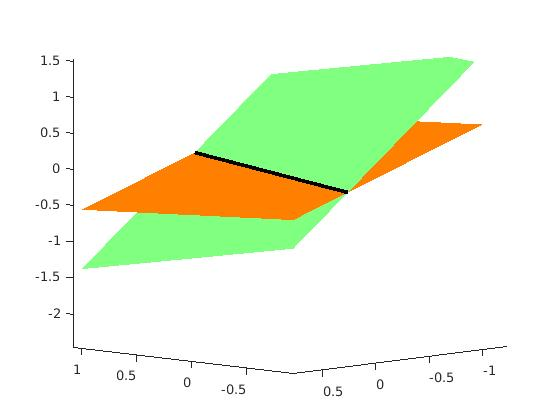
\includegraphics[width=0.5\textwidth]{planeintersection}
    \caption{The intersection between two planes can be found using linear algebra.}
    \label{fig:PlaneIntersection}
  \end{figure}
\end{ex}

\section{Matrix Algebra}
\begin{defn}[Matrix]
  A matrix is a rectangular array of \emph{entries}. If a matrix has $ n $ rows and $ m $ columns, we call
  it an $ n \times m$ matrix, where $ n $ and $ m $ are the \emph{dimensions} of the matrix.
\end{defn}
\begin{ex}
  \begin{displaymath}
    A = \begin{bmatrix} 3 & 2 \\ -4 & 1 \\ 0 & 1 \end{bmatrix}\quad
    B = \begin{bmatrix} 2 & 2 & -1 & -3 \\ 6 & 7 & 3 & 4 \\ -2 & 4 & 0 & 0 \end{bmatrix}\quad
    C = \begin{bmatrix} -1 & 0 & 8 & 2 \end{bmatrix}
  \end{displaymath}
  So $ A $ is a $ 3 \times 2 $ matrix, $ B $ is a $ 3 \times 4 $ matrix, and $ C $ is a $ 1 \times 4 $ matrix.
\end{ex}

\begin{defn}[Vector]
  A matrix with only one column is a \emph{column vector}; similarly, a matrix with only one row is
  a \emph{row vector}.
  \label{def:FormalVector}
\end{defn}

\begin{ex}
  The matrix $ C $ above is a row vector.
\end{ex}

We denote entries within a matrix using \emph{double subscript notation}.

\begin{ex}
  \begin{displaymath}
    D = \begin{bmatrix} d_{11} & d_{12} & d_{13} \\ d_{21} & d_{22} & d_{23} \end{bmatrix}
  \end{displaymath}
  The first subscript gives the row number, the second gives the column number.
\end{ex}

\begin{defn}[Matrix Sum]
  Let $ A $ and $ B $ be matrices with the same dimensions. Then $ A + B $ is
  the matrix obtained by adding corresponding entries of $ A $ and $ B $.
\end{defn}

\begin{ex}
  \begin{displaymath}
      \begin{bmatrix} 2 & 3 \\ 1 & -2 \end{bmatrix} + \begin{bmatrix} -2 & 4 \\ 2 & 3 \end{bmatrix}
    = \begin{bmatrix} 0 & 7 \\ 3 & 1 \end{bmatrix}.
  \end{displaymath}
\end{ex}

\begin{defn}[Multiplication by a Scalar]
  Let $ A $ be a matrix and $ \lambda $ be a scalar (number). Then the
  scalar multiple $ cA $ is the matrix obtained by multiplying each
  entry of $ A $ by $ c $.
\end{defn}

\begin{ex}
  \begin{displaymath}
    -2\begin{bmatrix} 3 & 2 & -1 \\ 6 & 1 & 7 \end{bmatrix} = \begin{bmatrix} -6 & -4 & 2 \\ -12 & -2 & -14 \end{bmatrix}
  \end{displaymath}
\end{ex}

\begin{defn}[Negative]
  The negative of a matrix $ A $, written as $ -A $, is simply the matrix $ (-1)A $
  and is obtained by reversing the signs of every entry in $ A $.
\end{defn}

\begin{defn}[Matrix Subtraction]
  $ A - B = A + -B $.
\end{defn}

\begin{defn}[Zero Matrix]
  The zero matrix $ O $ is any matrix consisting of only zero entries. $ A + O = O + A = A $ for
  any matrix $ A $. Obviously $ A - A = O $ for any matrix $ A $.
\end{defn}

Matrix multiplication is not simply the multiplication of corresponding entries.

\begin{defn}[Matrix Product]
  If $ A $ is an $ m \times n $ matrix and $ B $ is an $ n \times r $ matrix, the product
  $ C = AB $ is an $ m \times r $ matrix. The $ (i,j)$th entry of the product is given by
  $ c_{ij} = a_{i1}b_{1j} + a_{i2}b_{2j} + \cdots + a_{in}b_{nj} $.
\end{defn}

Note that $ A $ and $ B $ need not be the same size. However, the number of columns of $ A $ must
be the same as the number of rows of $ B $.

\begin{ex}
  \begin{displaymath}
    \begin{bmatrix} 1 & 3 & -1 \\ -2 & -1 & 1 \end{bmatrix}
    \begin{bmatrix} -4 & 0 & 3 & -1 \\ 5 & -2 & -1 & 1 \\ -1 & 2 & 0 & 6 \end{bmatrix} =
    \begin{bmatrix} 12 & -8 & 0 & -4 \\ 2 & 4 & -5 & 7 \end{bmatrix}
  \end{displaymath}
\end{ex}

\begin{ex}
  \begin{displaymath}
    \begin{bmatrix} 1 & 2 & 3 \\ 4 & 5 & 6 \\ 7 & 8 & 9 \end{bmatrix}
    \begin{bmatrix} x \\ y \\z \end{bmatrix} =
    \begin{bmatrix} x + 2y + 3z \\ 4x + 5y + 6z \\ 7x + 8y + 9z \end{bmatrix}
  \end{displaymath}
  \label{ex:VariableMultiply}
\end{ex}

Note that even if $ AB $ and $ BA $ are both defined, $ AB $ need not equal $ BA $ (matrix
multiplication is not commutative).

\begin{defn}[Matrix Powers]
  Let $ A $ be a square matrix. Then $ A^1 = A $, and $ A^n = \underbrace{AA \cdots A}_{n \text{ times}} $.
\end{defn}

\begin{figure}
    
\includegraphics[width=0.5\textwidth]{identitymatrix}
    \caption{Examples of the zero matrix and the identity matrix (\url{http://spikedmath.com/131.html}).}
    \label{fig:IdentityMatrix}
\end{figure}

\begin{defn}[Identity Matrix]
  The square $ n \times n $ matrix consisting solely of 1s on the diagonal and zeros elsewhere is
  called the identity matrix of order $ n $ and is denoted by $ I_n $ or simpy $ I $. We define
  $ A^0 = I $ for any square matrix $ A $.
\end{defn}

\begin{thm}
  If $ A $ is an $ n \times n $ square matrix, $ A I_n = I_n A = A $.
\end{thm}

\begin{ex}
  Let $ A = \begin{bmatrix} 2 & 3 \\ 5 & -1 \end{bmatrix} $. Then we have
  \begin{displaymath}
    \begin{bmatrix} 2 & 3 \\ 5 & -1 \end{bmatrix}\begin{bmatrix} 1 & 0 \\ 0 & 1 \end{bmatrix}= AI_2 = I_2A = A.
  \end{displaymath}
\end{ex}

\begin{defn}[Matrix Transpose]
  The transpose of the $ m \times n $ matrix $ A $ is the $ n \times m $ matrix $ A^T $ whose $ i$th column is the
  $ i$th row of $ A $.
\end{defn}

\begin{ex}
  \begin{displaymath}
    \begin{bmatrix} 1 & -1 \\ 2 & 0 \\ 3 & 4 \end{bmatrix}^T = \begin{bmatrix} 1 & 2 & 3 \\ -1 & 0 & 4 \end{bmatrix}
  \end{displaymath}
\end{ex}

\begin{thm}[Properties of Matrix Operations]
  Let $ A $, $ B $, and $ C $ be matrices with dimensions such that the following operations are defined, and
  let $ a $ and $ b $ be scalars. Then:
  \begin{enumerate}
    \item $ A + B = B + A $ (matrix addition is commutative)
    \item $ A + (B + C) = (A + B) + C $ (matrix addition is associative)
    \item $ A + O = A $ (addition of a matrix to the zero matrix gives same matrix)
    \item $ A + (-A) = O $ (addition of a matrix to its negative gives zero matrix)
    \item $ A(BC) = (AB)C $ (matrix multiplication is associative)
    \item $ AI = A = IA $ (multiplication by identity matrix gives same matrix)
    \item $ A(B + C) = AB + AC $ (matrix multiplication is distributive)
    \item $ (B + C)A = BA + CA $ (matrix multiplication is distributive)
    \item $ a(B + C) = aB + aC $ (scalar multiplication is distributive)
    \item $ (a + b)C = aC + bC $ (scalar multiplication is distributive)
    \item $ (ab)C = a(bC) $ (scalar multiplication is associative)
    \item $ 1A = A $ (multiplication by 1 gives same matrix)
    \item $ AO = O = OA $ (multiplication by zero matrix gives zero matrix)
    \item $ 0A = O $ (multiplication by zero scalar gives zero matrix)
    \item $ aO = O $ (scalar multiplication of zero matrix gives zero matrix)
    \item $ a(AB) = (aA)B = A(aB) $ (scalar multiplication commutes with matrix multiplication)
    \item $ (A + B)^T = A^T + B^T $ (transpose is linear with matrix addition)
    \item $ (AB)^T = B^T A^T $ (transpose is antilinear with matrix multiplication)
  \end{enumerate}
\end{thm}

\section{Inverse Matrices}
Return to example \ref{ex:VariableMultiply} from last lecture. This suggests we can write a set of linear
equations in the form $ Ax = b $ for some coefficient matrix $ A $, variable column vector $ x $, and column vector $ b $.

\begin{ex}
\begin{displaymath}\begin{array}{rllll}
  w & + x & + 2y & + 8z & = 2\\
  w &     & + y  &      & = 2\\
    & + x & + y  & + 4z & = -8\\
  w & - x &      &      & = 18
\end{array}\end{displaymath}
can be written as
\begin{displaymath}
  \begin{bmatrix} 1 & 1 & 2 & 8 \\ 1 & 0 & 1 & 0 \\ 0 & 1 & 1 & 4 \\ 1 & -1 & 0 & 0 \end{bmatrix}
  \begin{bmatrix} w \\ x \\ y \\ z \end{bmatrix}
  =
  \begin{bmatrix} 2 \\ 2 \\ -8 \\ 18 \end{bmatrix}
\end{displaymath}
\end{ex}

We now look for a general method to solve such an equation for $ x $ given $ A $ and $ b $.

Recall that we can solve $ ax = b $ as follows, where $ a $ and $ b $ are scalars:
\begin{displaymath}
  ax = b \implies a^{-1}ax = a^{-1} b \implies 1x = a^{-1} b \implies x = \frac{b}{a}
\end{displaymath}
Is there a similar way to solve matrix equations? In other words, for some matrix $ A $
is there a matrix $ A^{-1} $ such that
\begin{displaymath}
  Ax = b \implies A^{-1} Ax = A^{-1} b \implies Ix = A^{-1} b \implies x = A^{-1} b?
\end{displaymath}

We call such an $ A^{-1} $ the \emph{inverse} of $ A $.
\begin{defn}
  If $ A $ is an $ n \times n $ matrix, then the unique inverse of $ A $ (if it exists) is an
  $ n \times n $ matrix such that $ A A^{-1} = I_n = A^{-1} A $. If such an $ A^{-1} $
  exists, then $ A $ is called \emph{invertible}.
\end{defn}

\begin{ex}
 If we let $ A = \begin{bmatrix} 4 & 3 \\ 3 & 2 \end{bmatrix} $, then we have $ A^{-1} = \begin{bmatrix} -2 & 3 \\ 3 & -4 \end{bmatrix} $
 since $ A A^{-1} = I_3 = A^{-1} A $. Verify.
\end{ex}

\begin{ex}
  The matrix $ B = \begin{bmatrix} 3 & 2 \\ 9 & 6 \end{bmatrix} $ is \emph{not} invertible. Show.
\end{ex}

\begin{thm}
  If we have a linear system with coefficient matrix $ A $, variable vector $ x $, and constant vector $ b $,
  then the system has a unique solution if and only if $ A $ is invertible.  The unique solution vector is
  then given by $ A^{-1} b $ (noting that vector multiplication is not commutative).
\end{thm}

\begin{thm}[Inverse of $ 2 \times 2 $ matrices]
  If $ A = \begin{bmatrix} a & b \\ c & d \end{bmatrix} $ then $ A $ is invertible if and only if
  $ ad - bc \neq 0 $. If $ A $ is invertible, its inverse is given by
  \begin{displaymath}
    A^{-1} = \frac{1}{ad - bc}\begin{bmatrix} d & -b \\ -c & a \end{bmatrix}.
  \end{displaymath}
  We call the expression $ ad - bc $ the \emph{determinant} $ \det A $ of $ A $.
\end{thm}

\begin{ex}
  The inverse of $ A = \begin{bmatrix} 1 & 4 \\ 2 & 6 \end{bmatrix} $ is $ A^{-1} = \frac{1}{2} \begin{bmatrix} -6 & 4 \\ 2 & -1 \end{bmatrix} $.
\end{ex}

\begin{ex}
  The matrix $ B = \begin{bmatrix} 1 & 4 \\ 2 & 8 \end{bmatrix} $ is not invertible since $ \det B = 0 $.
\end{ex}

Finding the inverses of larger matrices is often much more computationally intensive. In fact, it is usually
more efficient to solve systems of equations using an elimination algorithm rather than by finding the inverse.
Elimination also works on rectangular matrices, while inverses can only be found for square matrices.

\begin{thm}
  Let $ A $ and $ B $ be invertible matrices, and let $ c $ be a non-zero scalar. Then
  \begin{enumerate}
    \item $ A^{-1} $ is invertible and $ (A^{-1})^{-1} = A $.
    \item $ cA $ is invertible and $ (cA)^{-1} = \frac{1}{c} A^{-1} $.
    \item $ AB $ is invertible and $ (AB)^{-1} = B^{-1} A^{-1} $.
    \item $ A^T $ is invertible and $ (A^T)^{-1} = (A^{-1})^T $.
    \item $ A^n $ is invertible for all non-negative integers $ n $, and $ (A^n)^{-1} = (A^{-1})^n $.
  \end{enumerate}
\end{thm}

\begin{ex}
  If $ A^{-1} (BX)^{-1} = (A^{-1} B^3))^2 $ then $ X = B^{-4} A B^{-3} $.
\end{ex}

So how do we, in general, find the inverse of some matrix if it has one?

\begin{thm}
  Let $ A $ be a square matrix. If a sequence of elementary row operations can reduce
  $ A $ to $ I $, then the same sequence of operations converts $ I $ to $ A^{-1} $.
\end{thm}

\begin{alg}[The Gauss-Jordan Method for Computing Inverses]
  Let $ A $ be an invertible $ n \times n $ matrix.
  \item Construct the "super-augmented" matrix $ [ A | I_n ] $.
  \item Row-reduce the augemented matrix so that it becomes $ [ I_n | B ] $.
  \item Then $ B = A^{-1} $.
\end{alg}

This algorithm is a consequence of the \emph{fundamental theorem of invertible
matrices}.
\begin{thm}[Fundamental Theorem of Invertible Matrices]
  Let $ A $ be an $ n \times n $ matrix. Then the following statements are equivalent:
  \begin{enumerate}
    \item $ A $ is invertible.
    \item $ Ax = b $ has a unique solution $ x $ for every $ b $.
    \item $ Ax = 0 $ has only the trivial solution $ x = 0 $.
    \item The reduced row echelon form of $ A $ is $ I_n $.
  \end{enumerate}
\end{thm}

This also implies that if $ A $ is not invertible, it cannot be reduced to $ I_n $. This
allows us to check invertibility of matrices.

\section{Vector Algebra}
Suppose an aeroplane is flying through the sky at a constant speed. There are four balanced
forces acting on the plane: weight, lift, thrust, and drag. Now, suppose that the aircraft
raises the nose into a climb; if the aircraft's thrust is not also increased, the plane will
actually begin to sink!

We can see why this is by drawing a \emph{vector diagram} showing the forces acting on the
plane while it is in both states.

\begin{defn}[Vector (informal)]
  A vector is a line segment with both length and direction.
\end{defn}

We often denote vectors with an arrow above their name, as in $ \overrightarrow{v} $.

We call a vector from point A to point B $ \overrightarrow{AB} $; $ A $ is called the \emph{tail}
and $ B $ the \emph{head}. We note that the position of a vector doesn't matter; only
the direction and length.

Each point $ A $ in the plane can be represented by the unique vector $ \overrightarrow{OA} $. We can therefore
represent that vector using the coordinates of the point. If $ A = (x, y) $, we write $ \overrightarrow{OA} = \begin{bmatrix} x \\ y \end{bmatrix} $.
This notation should be familiar from definition \ref{def:FormalVector}.

\begin{defn}[Real coordinate space]
  Define the real coordinate space of dimension $ n $, notated by $ \mathbb{R}^n $, to be
  the set of all vectors with $ n $ real components.
\end{defn}

\begin{ex}
  So $ \mathbb{R}^2 $ is the coordinate plane. We have $ [2, 3] \in \mathbb{R}^2 $.
\end{ex}

\begin{ex}
  Three-dimensional space is called $ \mathbb{R}^3 $. We have $ [1, 0, 0] \in \mathbb{R}^3 $.
\end{ex}

Vector addition, subtraction, and multiplication by scalars have the same meaning as that for
matrices. However, we can look at them geometrically (see figure \ref{fig:VectorAddition}).

\begin{figure}
  
\includegraphics[width=0.5\textwidth]{vectors}
  \caption{The parallelogram rule for adding vectors.}
  \label{fig:VectorAddition}
\end{figure}

\begin{ex}
  \begin{align*}
    \begin{bmatrix} 3 \\ 2 \end{bmatrix} + \begin{bmatrix} 7 \\ 2 \end{bmatrix} &= \begin{bmatrix} 10 \\ 4 \end{bmatrix}\\
    \begin{bmatrix} 3 \\ 2 \end{bmatrix} - \begin{bmatrix} 7 \\ 2 \end{bmatrix} &= \begin{bmatrix} -4 \\ 0 \end{bmatrix}
  \end{align*}
  (Draw both.)
\end{ex}

\begin{ex}
  \begin{align*}
    6\begin{bmatrix} 1 \\ 2 \end{bmatrix} &= \begin{bmatrix} 6 \\ 12 \end{bmatrix}\\
    3\begin{bmatrix} 6 \\ 2 \\ -1 \\ 3 \\ -3 \\ 30 \end{bmatrix} &= \begin{bmatrix} 18 \\ 6 \\ -3 \\ 9 \\ -9 \\ 90 \end{bmatrix}
  \end{align*}
  (Draw first. Note the second is still a valid vector in $ \mathbb{R}^6 $.)
\end{ex}

\begin{defn}[Linear combination]
  A vector $ v $ is a linear combination of vectors $ v_1, v_2, \dots, c_n $ iff there
  are scalars $ \alpha_1, \alpha_2, \dots, \alpha_n $ such that
  \begin{displaymath}
    v = \alpha_1 v_1 + \alpha_2 v_2 + \cdots + \alpha_n v_n.
  \end{displaymath}
\end{defn}

\begin{ex}
  The vector $ [17, -12, 20]^T $ is a linear combination of $ [3, 2, 0]^T $, $ [7, 0, 3]^T $, and $ [0, 0, 5]^T $
  since:
  \begin{displaymath}
   \begin{bmatrix} 17 \\ -12 \\ 20 \end{bmatrix} = -6 \begin{bmatrix} 3 \\ 2 \\ 0 \end{bmatrix}
                                                   +5 \begin{bmatrix} 7 \\ 0 \\ 3 \end{bmatrix}
                                                   +  \begin{bmatrix} 0 \\ 0 \\ 5 \end{bmatrix}.
  \end{displaymath}
\end{ex}

In $ \mathbb{R}^2 $, all vectors are linear combinations of $ e_1 = \begin{bmatrix} 1 \\ 0 \end{bmatrix} $ and $ e_2 = \begin{bmatrix} 0 \\ 1 \end{bmatrix} $.
Similarly, in $ \mathbb{R}^3 $ all vectors are linear combinations of
\begin{displaymath}
  e_1 = \begin{bmatrix} 1 \\ 0 \\ 0 \end{bmatrix} \text{, }
  e_2 = \begin{bmatrix} 0 \\ 1 \\ 0 \end{bmatrix} \text{, and }
  e_3 = \begin{bmatrix} 0 \\ 0 \\ 1 \end{bmatrix}.
\end{displaymath}
These special vectors are called the \emph{standard basis vectors}. In physics and
engineering, $ \hat i $, $ \hat j $, and $ \hat k $ are often used to denote $ e_1 $, $ e_2 $,
and $ e_3 $ respectively. In effect, they define the coordinate plane.

\section{Dot Product}
Suppose $ u $ and $ v $ are row vectors in $ \mathbb{R}^n $. Since they are matrices, we can define
the multiplication $ u \bullet v = u v^T $ (transposing the second matrix to become a column matrix
so that the multiplication is defined). For column vectors, we define $ u \bullet v = u^T v $.

This product is known as the \emph{dot product}, and has several useful geometric properties. With
some trivial calculation, it can be shown that a more easily applicable of the dot product exists:

\begin{thm}[Dot Product II]
  Suppose $ u $ and $ v $ are row vectors in $ \mathbb{R}^n $ such that $ u = [u_1, u_2, \dots, u_n] $
  and $ v = [v_1, v_2, \dots, v_n] $. Then $ u \bullet v = u_1v_1 + u_2v_2 + \cdots + u_nv_n $.
  \label{thm:EasyDotty}
\end{thm}

Note that the dot product takes two vectors and returns a scalar, \emph{\textbf{not another vector}}. The dot
product is also defined in the same way for column vectors (the addition together of the product of corresponding
components).

\begin{ex}
  $ \begin{bmatrix} 2 \\ 3 \end{bmatrix} \bullet \begin{bmatrix} 5 \\ -5 \end{bmatrix} = 10 - 15 = -5. $
\end{ex}

While matrix multiplication is not commutative ($ XY \neq YX $ in general), it can easily be shown using
the definition in theorem \ref{thm:EasyDotty} that the dot product \emph{is} commutative. This, and
several other properties, are described in the following theorem.

\begin{thm}[Dot Product Properties]
  Let $ u, v, w \in \mathbb{R}^n $ be vectors, and let $ \alpha $ be a scalar. Then:
  \begin{enumerate}
    \item $ u \bullet v = v \bullet u $
    \item $ u \bullet (v + w) = u \bullet v + u \bullet w $
    \item $ (\alpha u) \bullet v = \alpha(u \bullet v) $
    \item $ u \bullet u \geq 0 $
    \item $ u \bullet u = 0 $ iff $ u = 0 $
  \end{enumerate}
\end{thm}

To formally define the "length" of a vector in $ n $ dimensions, we have:
\begin{defn}[Relationship of Length to Dot Product]
  If $ v $ is a vector then $ u \bullet u = \norm{u}^2 $, where
  $ \norm{u} $ is the \emph{norm} or \emph{length} of $ u $.
\end{defn}

Note that the definition of "length" given here agrees with Pythagoras' Theorem,
as the following example suggests.

\begin{ex}
  We will calculate the length of $ v = [13, 84] $ using the dot product:
  \begin{displaymath}
    \norm{u} = \sqrt{v \bullet v} = \sqrt{13 \times 13 + 84 \times 84} = 85
  \end{displaymath}
  So the dot product formula for length seems to simply reduce to Pythagoras' Theorem
  (and it can easily be proved that this is, in fact, the case)!
\end{ex}

Some common-sense results follow:
\begin{thm}[Length Properties]
  Let $ v \in \mathbb{R}^n $ be a vector, and let $ \alpha $ be a scalar. Then:
  \begin{enumerate}
    \item $ \norm{v} = 0 \iff v = 0 $
    \item $ \norm{\alpha v} = \abs{\alpha}\norm{v} $
  \end{enumerate}
\end{thm}

If a vector has a length of 1, it is called a \emph{unit vector}. The process of finding the
unique unit vector in the same direction as some vector $ v $ is known as \emph{normalising}
the vector, and is carried out simply by dividing $ v $ by its own length, $ \norm{v} $.

We define the \emph{distance} between two vectors to be the length of the vector which joins
their two heads. Looking back at the parallelogram diagram from last lecture (figure \ref{fig:VectorAddition}),
we have the following definition:
\begin{defn}[Distance between two vectors]
  The distance $ \dis(u, v) $ between two vectors $ u, v \in \mathbb{R}^n $ is defined as
  $ \dis(u,v) = \norm{u - v} $.
\end{defn}

\begin{ex}
  The distance between $ u = \begin{bmatrix} 3 \\ 4 \end{bmatrix} $ and $ v = \begin{bmatrix} 7 \\ 9 \end{bmatrix} $
  will be:
  \begin{align*}
    \dis(u,v) = \norm{u - v} &= \norm{\begin{bmatrix} -4 \\ -5 \end{bmatrix}}\\
                             &= \sqrt{16 + 25} \\
                             &= \sqrt{41} \approx 6.4
  \end{align*}
\end{ex}

Having seen how the dot product relates to the length of a vector, we now turn to the problem
of direction --- how do we find the angle between two vectors? After some computation, we
find the following third expression of the dot product:

\begin{thm}[Dot Product III]
  Suppose $ u, v \in \mathbb{R}^n $ are vectors, and that the angle between them is $ \theta $.
  Then $ u \bullet v = \norm{u} \norm{v} \cos \theta $.
  \label{thm:DotProductCosine}
\end{thm}
\begin{figure}
  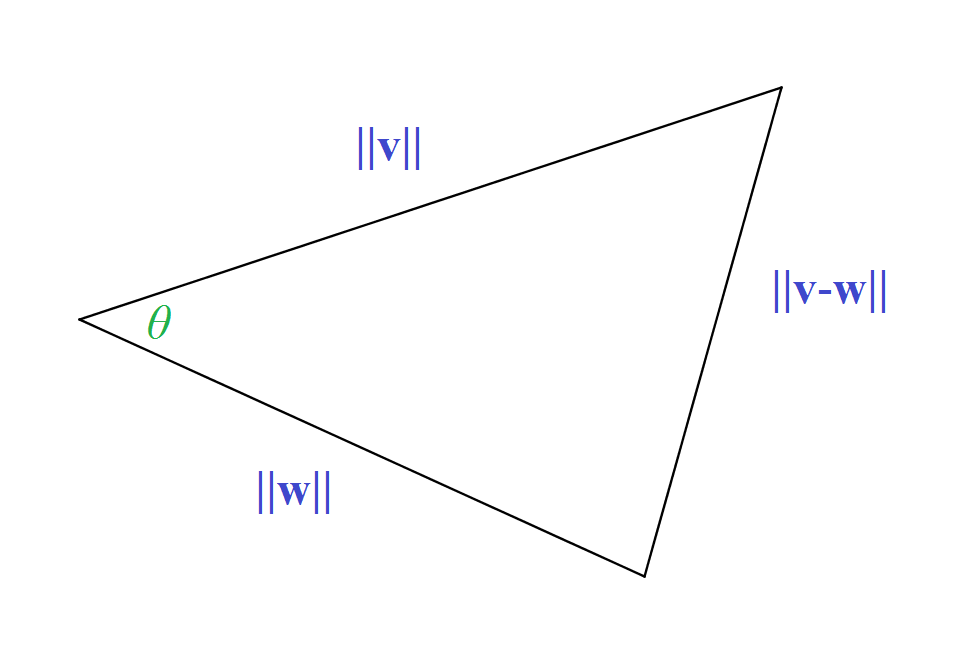
\includegraphics[width=0.5\textwidth]{cosinelaw}
  \caption{Notation for proof of theorem \ref{thm:DotProductCosine}.}
  \label{fig:DotProductCosine}
\end{figure}
\begin{proof}
  See figure \ref{fig:DotProductCosine}. We have, via the cosine law, the following:
  \begin{align*}
    \norm{u}^2 + \norm{v}^2 - 2\norm{u}\norm{v} \cos \theta &= \norm{u-v}^2\\
                                                            &= u \bullet u - 2(u \bullet v) + v \bullet v \\
                                                            &= \norm{u}^2 - 2(u \bullet v) + \norm{v}^2\\
                                                            &\Downarrow\\
                            - 2\norm{u}\norm{v} \cos \theta &=            - 2(u \bullet v)\\
                                                            &\Downarrow\\
                               \norm{u}\norm{v} \cos \theta &= u \bullet v
  \end{align*}
\end{proof}

If two vectors $ u $ and $ v $ are at right angles, $ \cos \theta = 0 $ so $ u \bullet v = 0 $ and $ u $ and $ v $ are called \emph{orthogonal}.

\begin{ex}
  The angle between $ [3, 4, 5] $ and $ [2, -1, 6] $ is around $ 45^{\circ} $.
\end{ex}

\begin{ex}
  The vectors $ [0, 3, 0] $ and $ [1, 0, 0] $ are orthogonal.
\end{ex}

\begin{thm}[Pythagoras' Theorem (optional)]
  Let $ u, v \in \mathbb{R}^n $ such that $ u \bullet v = 0 $. Then $ \norm{u+v}^2 = \norm{u}^2 + \norm{v}^2 $.
\end{thm}
\begin{proof}
  \begin{align*}
    \norm{u+v}^2 &= (u + v) \bullet (u + v)\\
                 &= u \bullet (u + v) + v \bullet (u + v)\\
                 &= u \bullet u + u \bullet v + v \bullet u + v \bullet v\\
                 &= \norm{u}^2 + 2(u \bullet v) + \norm{v}^2\\
                 &= \norm{u}^2 + 2\times0 + \norm{v^2}\\
                 &= \norm{u}^2 + \norm{v}^2.
  \end{align*}
\end{proof}

We can also find the \emph{projection} of one vector on another using the dot product.
The projection of one vector on another is simply the "shadow" of the vector --- the
component of the vector in the same direction as the vector it is being projected onto.

\begin{thm}[Projection]
  The projection of the vector $ a $ on the vector $ v $ is given by
  \begin{displaymath}
    \vectorproj[v]{a} = \left(\frac{a \bullet v}{v \bullet v}\right) v.
  \end{displaymath}
\end{thm}

\section{Matrix Transformations}
We have seen that the geometric meaning of vectors is a point in space. Now, we see that
matrices are \emph{transformations} which act on a space itself, shifting each point (vector)
in that space around. In fact, matrices act as \emph{linear} transformations (which are slightly
more restrictive in terms of their behaviour than general transformations).

The main idea behind this is the observation that the multiplication of any $ n \times n $
matrix by a column vector in $ \mathbb{R}^n $ gives another column vector of the same "flavour".

\begin{ex}
  Suppose $ A = \begin{bmatrix} 2 & 3 \\ 3 & 3 \end{bmatrix} $ and $ \vec{x} = \begin{bmatrix} 1 \\ 1 \end{bmatrix} $.
  Then $ A\vec{x} = \begin{bmatrix} 5 \\ 6 \end{bmatrix} = \vec{x}' $. Graphically, $ A $ transforms $ \vec{x} $
  to $ \vec{x}' $ as in figure \ref{fig:FirstMatrixTransform}.

  \begin{figure}
    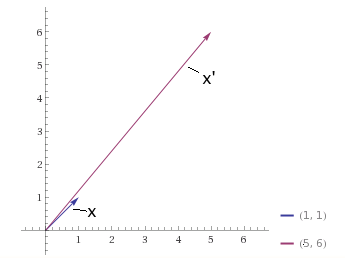
\includegraphics[width=0.5\textwidth]{mtransform1}
    \caption{The matrix $ A $ maps $ \vec{x} $ to $ \vec{x}' $.}
    \label{fig:FirstMatrixTransform}
  \end{figure}
\end{ex}

We can be more specific about what exactly a transformation matrix "does" with each point,
by noting that each point in $ \mathbb{R}^n $ is a linear combination of the standard basis
vectors. This means we only need to care about where the matrix sends the standard basis
vectors, since we can reconstruct the rest of the space around them.

Luckily we chose our standard basis vectors well, and so we state the following theorem
(which is easy to show):

\begin{thm}[Transformation of Basis Vectors]
  Suppose $ A $ is an $ n \times n $ matrix. Then $ A e_i $ is simply the $ i$th
  column of $ A $. In other words, the columns of the matrix corresponding to a transformation
  are simply the images of the standard basis vectors under that transformation.
\end{thm}

\begin{ex}
  If we have a transformation $ T : \mathbb{R}^2 \rightarrow \mathbb{R}^2 $ that sends $ e_1 \leadsto \begin{bmatrix} 1 \\ 2 \end{bmatrix} $
  and $ e_2 \leadsto \begin{bmatrix} 0 \\ 2 \end{bmatrix} $ then the corresponding matrix is $ A_T = \begin{bmatrix} 1 & 0 \\ 2 & 2 \end{bmatrix} $.
\end{ex}

Once we have mapped our basis vectors, we obtain a \emph{new coordinate system} which can
be used to map all the other vectors in our space.

Why is this useful? It allows us to transform sets of numbers in complicated ways efficiently
(e.g. in graphics or gaming software, or for simulations). We can represent rotations, skews,
projections, and translations of spaces using a single object.

\begin{ex}[Reflection]
  One transformation which we can perform is a reflection of our space across the line $ y = x $.
  This transformation will send $ e_1 $ to $ e_2 $ and vice versa, so it corresponds to the matrix
  \begin{displaymath}
    T_R = \begin{bmatrix} 0 & 1 \\ 1 & 0 \end{bmatrix}.
  \end{displaymath}

  This transformation sends $ \vec{x} = \begin{bmatrix} 3 \\ 4 \end{bmatrix} $ to $ T_R \vec{x} = \begin{bmatrix} 4 \\ 3 \end{bmatrix} $.
\end{ex}

\begin{ex}[Scale]
  If we grow or shrink all vectors in our space by a factor of $ r $, we have a linear transformation which
  is respectively known as a dilation or contraction. This transformation sends $ e_1 \leadsto re_1 $
  and $ e_2 \leadsto re_2 $, so the corresponding matrix is
  \begin{displaymath}
    T_D = \begin{bmatrix} r & 0 \\ 0 & r \end{bmatrix}.
  \end{displaymath}
\end{ex}

\begin{ex}[Rotation]
  If we rotate our plane around the origin by an angle of $ \theta $, we obtain the linear
  transformation with a corresponding matrix
  \begin{displaymath}
    T_\theta = \begin{bmatrix} \cos \theta & -\sin \theta \\ \sin \theta & \cos \theta \end{bmatrix}.
  \end{displaymath}
\end{ex}

\begin{ex}[Shear]
  If we send the vector $ (x, y) \leadsto (x + 2y, y) $, we obtain a space which
  is "slanted". This example has the corresponding matrix $ \begin{bmatrix} 1 & 2 \\ 0 & 1 \end{bmatrix} $;
  in general, any shear matrix looks like
  \begin{displaymath}
    T_S = \begin{bmatrix} 1 & m \\ n & 1 \end{bmatrix}
  \end{displaymath}
  where $ m $ is the shear factor in the $ x $ direction, and $ n $ is the shear factor in
  the $ y $ direction. See figure \ref{fig:Shear}.

  \begin{figure}
    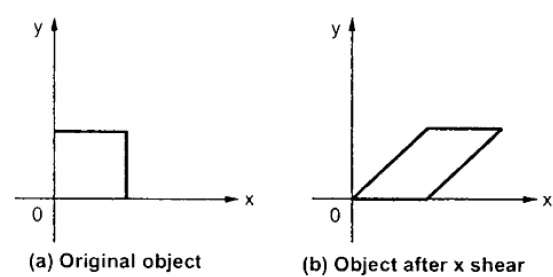
\includegraphics[width=0.6\textwidth]{710_shear_x}
    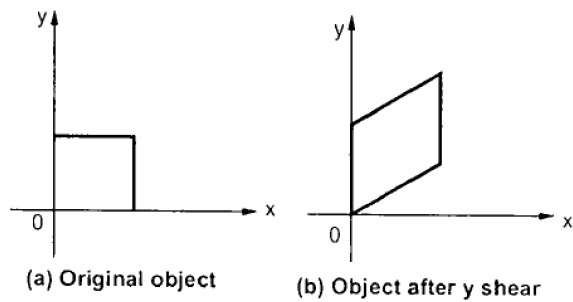
\includegraphics[width=0.6\textwidth]{710_shear_y}
    \caption{Shearing transformations.}
    \label{fig:Shear}
  \end{figure}
\end{ex}

\begin{ex}[Projection]
  The transformation which sends each vector to its projection on a specific
  vector is also linear. Suppose that we want to project our space onto the vector $ v = (x,y)^T $.

  Then we have
  \begin{displaymath}
    T_\pi (e_1) = \vectorproj[v]{e_1} = \frac{e_1 \bullet v}{v \bullet v} \begin{bmatrix} x \\ y \end{bmatrix}
                                      = \frac{x}{x^2 + y^2} \begin{bmatrix} x \\ y \end{bmatrix},
  \end{displaymath}
  and likewise
  \begin{displaymath}
    T_\pi (e_2) = \vectorproj[v]{e_2} = \frac{e_2 \bullet v}{v \bullet v} \begin{bmatrix} x \\ y \end{bmatrix}
                                      = \frac{y}{x^2 + y^2} \begin{bmatrix} x \\ y \end{bmatrix}.
  \end{displaymath}

  Hence
  \begin{displaymath}
    T_\pi = \begin{bmatrix} \frac{x^2}{x^2 + y^2} & \frac{xy}{x^2 + y^2} \\ \frac{xy}{x^2 + y^2} & \frac{y^2}{x^2 + y^2} \end{bmatrix}.
  \end{displaymath}

  Note that $ \det{T_\pi} = 0 $ for all $ x $ and $ y $, and so projection transformations are not invertible.
  This makes sense, as we can send multiple vectors to the same point on the line, and so we cannot know which
  vector to send that point back to.
\end{ex}

To do multiple transformations one after the other, we simply multiply the corresponding matrices.

\begin{ex}
  To perform a $ 90^\circ $ rotation followed by a $ 2 \times $ dilation, we multiply the
  matrices together right-to-left:
  \begin{align*}
    T = T_D T_{90^\circ} &= \begin{bmatrix} 2 & 0 \\ 0 & 2 \end{bmatrix} \begin{bmatrix} 0 & -1 \\ 1 & 0 \end{bmatrix} \\
                         &= \begin{bmatrix} 0 & -2 \\ 2 & 0\end{bmatrix}.
  \end{align*}
\end{ex}

\section{Determinants}
Last time, we saw that matrices are \emph{transformations} which act on spaces, transforming
vectors into other vectors. In this lecture, we will consider square matrices, which move
vectors around without changing the dimensions of the space.

How can we tell when a matrix is \emph{invertible}? Well, a matrix must be invertible if and
only if the corresponding transformation is invertible --- i.e. if, for every output vector, we can
\emph{uniquely identify} the input vector which was transformed to it. Obviously, this implies
that non-invertible matrices will send multiple distinct vectors to each single output.

For this to happen, the matrix must send the basis vectors "into line" with each other (i.e. in 2D space, the
two basis vectors will be sent to the same line; in 3D space, the three basis vectors will be sent to the same
plane or to the same line; and in $n$D space, the $ n $ basis vectors will be sent to a subspace of dimension
$ n - 1 $). In other words, \emph{the area enclosed by the image of the unit cube under the transformation will
become zero}.

The area/volume/hypervolume of the image of the unit cube under some matrix transformation $ A $ is known
as the \emph{determinant} $ \det A $. The sign of the determinant indicates whether the basis vectors have
swapped places.

The standard way to calculate determinants of a matrix is to `expand' a matrix along a row
or a column as in the following theorem.

\begin{thm}[Laplace Expansion]
  The determinant of any square $ n \times n $ matrix $ A = [a_ij] $ can be calculated as follows:
  \begin{displaymath}
    \det A = a_{i1} C_{i1} + a_{i2} C_{i2} + \cdots + a_{in} C_{in},
  \end{displaymath}
  where each $ C_{ij} $ is the $ (i,j)$-cofactor of $ A $,
  \begin{displaymath}
    C_ij = (-1)^{i+j} \det A_{ij},
  \end{displaymath}
  where $ A_{ij} $ is the matrix obtained by deleting the $ i$th row and $ j$th column of $ A $.
  The signs of each cofactor can be remembered easily by noting that they form a checkerboard pattern.
\end{thm}

\begin{ex}
  \begin{align*}
    \det \begin{bmatrix} 7 & 4 & 2 \\ 6 & 6 & 2 \\ 7 & 9 & 0 \end{bmatrix}
      &= 7 \det \begin{bmatrix} 6 & 2 \\ 9 & 0 \end{bmatrix} - 4 \det \begin{bmatrix} 6 & 2 \\ 7 & 0 \end{bmatrix}
       + 2 \det \begin{bmatrix} 6 & 6 \\ 7 & 9 \end{bmatrix}\\
      &= 7(6-18) - 4(-14) + 2(54-63)\\
      &= -46.
  \end{align*}
\end{ex}

The following two theorems, in combination with row reduction, are often an easier method.

\begin{thm}
  The determinant of an upper-triangular matrix is simply the product of the diagonal entries.
\end{thm}

\begin{ex}
  \begin{align*}
    \det \begin{bmatrix} 3 & 5 & 5 \\ 0 & 0 & 3 \\ 0 & 0 & 1 \end{bmatrix} &= 3 \times 0 \times 1 = 0.\\
    \det \begin{bmatrix} 4 & 72 & 1000 & 37 \\ 0 & 4 & 63 & -200 \\ 0 & 0 & 2 & 666 \\ 0 & 0 & 0 & 420 \end{bmatrix} &= 4 \times 4 \times 2 \times 420 = 13440.
  \end{align*}
\end{ex}

\begin{thm}
  Let $ A $ be a square matrix. Then
  \begin{enumerate}
    \item If $ A $ has a zero row or a zero column, then $ \det A = 0 $.
    \item If a square matrix $ B $ is obtained by exchanging two rows or columns of $ A $, then $ \det B = -\det A $.
    \item If $ A $ has two identical rows or columns, then $ \det A = 0 $.
    \item If $ B $ is obtained by multiplying a single row or column of $ A $ by a scalar $ k $, then $ \det B = k\det A $.
    \item If $ A $, $ B $, and $ C $ are identical square matrices except that a row or column of $ A $ is the sum
          of the corresponding rows of $ B $ and $ C $, then $ \det A = \det B + \det C $.
    \item If $ B $ is obtained by adding a multiple of one row (or column) of $ A $ to another, then $ \det B = \det A $.
    \item If $ A $ is an $ n \times n $ square matrix, then $ \det (kA) = k^n \det A $.
    \item If $ A $ and $ B $ have the same dimensions, then $ \det (AB) = \det A \det B $.
    \item If $ A $ is invertible, then $ \det A^{-1} = (\det A)^{-1}$.
    \item If $ A^T $ is the transpose of $ A $, then $ \det A^T = \det A $.
  \end{enumerate}
\end{thm}

Our main reason for studying determinants is that they have an application to eigen-calculations; however, they
do have some nice properties. One (impractical) application of determinants is curve fitting.

Suppose that $ (x_1, y_1) $ and $ (x_2, y_2) $ are points on a plane, and we wish to fit a linear
equation to them. Then we are attempting to solve the following system of equations:
\begin{align*}
  a x_1 + b y_1 + c &= 0\\
  a x_2 + b y_2 + c &= 0,
\end{align*}
which has a coefficient matrix
\begin{displaymath}
  A = \begin{bmatrix} x_1 & y_1 & 1 \\ x_2 & y_2 & 1 \end{bmatrix}.
\end{displaymath}

Recall that the fundamental theorem of invertible matrices stated that $ Ax = 0 $ has only the trivial solution $ x = 0 $
if and only if $ A $ is invertible. Now, this system obviously does not have only the trivial solution (since $ a $, $ b $,
and $ c $ are not all zero), and so $ A $ cannot be invertible. Hence $ \det A = 0 $, and the equation
of the line through the points is given by
\begin{displaymath}
  \det \begin{bmatrix} x_1 & y_1 & 1 \\ x_2 & y_2 & 1 \end{bmatrix} = 0.
\end{displaymath}

\section{Markov Chains}
\begin{ex}
  Suppose that each year 15\% of the non-Wellingtonian New Zealand population migrates to Wellington, and 10\%
  of Wellingtonians migrate out of Wellington. Suppose further that there is no net migration into
  or out of the country.

  Suppose that in year 0, the proportion of the NZ population living in Wellington is $ x_0 $
  and the proportion of the NZ population not living in Wellington is $ 1 - x_0 = y_0 $.
  We therefore have that in year 1, $ x_1 = 0.9x_0 + 0.15y_0 $ and $ y_1 = 0.1x_0 + 0.85y_0 $.

  In general, we have the following set of equations for the $ n + 1$th year:
  \begin{align*}
    x_{n+1} = 0.9x_n + 0.15y_n\\
    y_{n+1} = 0.1x_n + 0.85y_n
  \end{align*}
  Or, writing
  \begin{displaymath}
    X_n = \begin{bmatrix} x_n \\ y_n \end{bmatrix} \text{ and } A = \begin{bmatrix} 0.9 & 0.15 \\ 0.1 & 0.85 \end{bmatrix}
  \end{displaymath}
  we have $ X_{n+1} = AX_n $.

  What will the final population distribution be? Taking the limit as $ n \to \infty $ of $ X_{n+1} = AX_n $,
  we obtain $ X = AX $.
  We therefore have the following chain of reasoning:
  \begin{align*}
    \begin{bmatrix} 0.9 & 0.15 \\ 0.1 & 0.85 \end{bmatrix} \begin{bmatrix} x \\ y \end{bmatrix} &= \begin{bmatrix} x \\ y \end{bmatrix}\\
    \begin{bmatrix} -0.1 & 0.15 \\ 0.1 & -0.15 \end{bmatrix} \begin{bmatrix} x \\ y \end{bmatrix} &= \begin{bmatrix} 0 \\ 0 \end{bmatrix}\\
    \begin{bmatrix} -0.1 & 0.15 \\ 0 & 0 \end{bmatrix} \begin{bmatrix} x \\ y \end{bmatrix} &= \begin{bmatrix} 0 \\ 0 \end{bmatrix}
  \end{align*}
  So $ \begin{bmatrix} x \\ y \end{bmatrix} = t\begin{bmatrix} 0.15 \\ 0.1 \end{bmatrix} $ for some parameter $ t $. We can identify what this parameter is,
  because we want the two entries to add to 1 (they are probabilities); hence $ t = \frac{1}{0.15 + 0.1} = \frac{1}{0.25} $ and so
  $ \begin{bmatrix} x \\ y \end{bmatrix} = \begin{bmatrix} 0.6 \\ 0.4 \end{bmatrix} $. So, in the long run, 60\% of the New Zealand population will
  live in Wellington and 40\% will not. What fun, and excitement!
  \label{ex:Markov}
\end{ex}

\begin{defn}[Markov Process]
  This is an example of a \emph{Markov process}: a system with some finite set of states such that at each instant the system
  has a well-defined state, and over a fixed period of time it changes to another state (the probabilities of doing so being
  constant).
\end{defn}

\begin{defn}[Probability Vector]
  A vector whose entries add to 1.
\end{defn}

\begin{ex}
  $ v = \begin{bmatrix} 0.2 \\ 0.3 \\ 0.5 \end{bmatrix} $ is a probability vector.
\end{ex}

\begin{defn}[Stochastic Matrix]
  A stochastic matrix is a matrix whose columns are probability vectors.
\end{defn}

In example \ref{ex:Markov}, the vector which we found as we let $ n \to \infty $ is known as a \emph{steady state vector}.

\begin{defn}[Steady-State Vector]
  If $ P $ is a stochastic matrix, a steady-state vector (or \emph{equilibrium vector}) of $ P $ is
  some probability vector $ v_\infty $ such that $ Pv_\infty = v_\infty $.
\end{defn}

\begin{alg}[Finding a Steady-State Vector]
  Suppose $ P $ is the stochastic matrix for which we wish to find a steady-state vector $ v_\infty $. We proceed as follows:
  \begin{enumerate}
    \item Rearrange $ Pv = v $:
      \begin{align*}
        Pv &= v\\
        Pv - v &= 0\\
        Pv - Iv &= 0\\
        (P - I)v &= 0
      \end{align*}
    \item Row-reduce $ P - I $ to find a non-zero solution for $ v $ (setting the parameter arbitrarily).
    \item Divide $ v $ by the sum of its entries to convert it into a probability vector, $ v_\infty $.
  \end{enumerate}
\end{alg}

\begin{thm}
  If $ P $ is a stochastic matrix such that some power of $ P $ contains only non-zero entries,
  then it has a unique steady-state vector which it converges to \emph{regardless of the inital state}.
\end{thm}

Another example:

\begin{ex}
  \begin{figure}
    
\includegraphics[width=0.5\textwidth]{invercargill}
    \caption{The city centre of Invercargill.}
    \label{fig:PlaneIntersection}
  \end{figure}
  Invercargill (a small remote village in New Zealand) receives radio broadcasts from both Radio New Zealand
  stations, Radio New Zealand National ($ N $) and Radio New Zealand Concert ($ C $). Of the listers tuned
  to RNZ National, 70\% will remain listening to it after the regular power cut which occurs in Invercargill
  every 30 minutes (on the hour and on the half hour) and 30\% will switch to listening to RNC Concert. Of
  the listeners tuned to the concert station, 60\% will switch to listening to RNZ National and only 40\%
  will continue listening to the concert. Since there is no other entertainment available in Invercargill,
  no-one ever switches off the radio. Suppose that at 8:15 AM, all listeners are listening to RNZ National,
  so our initial state vector will be $ v_0 = \begin{bmatrix} 1 \\ 0 \end{bmatrix} $.

  We have the following system of equations:
  \begin{align*}
    N_{n+1} &= 0.7N_n + 0.6C_n\\
    C_{n+1} &= 0.3N_n + 0.4C_n
  \end{align*}
  And therefore we have the stochastic matrix $ P = \begin{bmatrix} 0.7 & 0.6 \\ 0.3 & 0.4 \end{bmatrix} $.

  At 9:25 AM, two power cuts will have occurred (one at 8:30, and one at 9:00). Hence, the state
  vector will be
  \begin{displaymath}
    v_2 = P^2 v_0 = \begin{bmatrix} 0.67 & 0.66 \\ 0.33 & 0.34 \end{bmatrix} \begin{bmatrix} 1 \\ 0 \end{bmatrix} = \begin{bmatrix} 0.67 \\ 0.33 \end{bmatrix}.
  \end{displaymath}

  As $ n \to \infty $, we will have $ v_\infty = \begin{bmatrix} \frac{2}{3} \\ \frac{1}{3} \end{bmatrix} $.
\end{ex}

\section{Eigen Calculations}
We saw last time that some vectors have the property that when they are acted upon by a matrix, they do not change. We
called vectors with this property "steady-state vectors". In this lecture, we generalise this idea.

\begin{defn}[Eigenvector]
  Let $ A $ be a square matrix. A vector $ x $ is an eigenvector if $ Ax = \lambda x $ for some scalar $ \lambda $.
  The multiplying factor $ \lambda $ is called an \emph{eigenvalue} of the matrix.
\end{defn}

In particular, a steady-state vector is an eigenvector with an eigenvalue of 1.

\begin{ex}
  All $n$-vectors are eigenvectors of the $n \times n $ identity matrix.
\end{ex}

\begin{ex}
  \begin{displaymath}
    \begin{bmatrix} 3 & 2 \\ 6 & 4 \end{bmatrix} \begin{bmatrix} 1 \\ 2 \end{bmatrix} = \begin{bmatrix} 7 \\ 14 \end{bmatrix} = 7\begin{bmatrix} 1 \\ 2 \end{bmatrix}
  \end{displaymath}
\end{ex}

\end{document}
